\section<presentation>[NetFilter]{Fonctionnement de NetFilter}
  \begin{frame}
    \frametitle{Architecture G�n�rale}
    \begin{figure}
      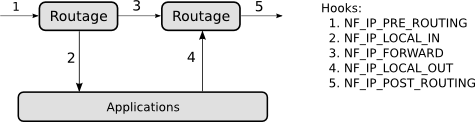
\includegraphics[scale=0.7]{pictures/netfilter.png}
    \end{figure}
  \end{frame}

  \begin{frame}
    \frametitle{Iptables: Principes}
    Fonctions: Regrouper en tables des r�gles de filtrage et de
    modification de paquets IP.

    \begin{center}
      \begin{tabular}{|l|l|}
	\hline
	\textbf{Table} & \textbf{Hooks} \\
	\hline
	filter & INPUT, OUTPUT, FORWARD \\
	\hline
	nat & PREROUTING, POSTROUTING \\
	\hline
	mangle & Toutes \\
	\hline
      \end{tabular}
    \end{center}

  \end{frame}

  \begin{frame}
    \frametitle{Iptables: Exemples}
    \begin{itemize}
    \item Filter: \\ 
      {\tt\scriptsize iptables -t filter -A INPUT -p tcp --dport 80 -j DROP}
    \item Nat: \\
      {\tt\scriptsize iptables -t nat -A POSTROUTING -d ! 192.168.0.0/24 -j
      SNAT --to-source 81.57.230.21}
    \item Mangle: \\
      {\tt\scriptsize iptables -t mangle -A POSTROUTING -p udp --dport 53 -j TOS --set-tos 16}
    \end{itemize}
  \end{frame}

  \begin{frame}
    \frametitle{Conntrack}
    Principe: 
    \begin{itemize}
    \item Regrouper les paquets en flux � partir des triplets (IP
    source, port source, port destination)
    \item Associer � chaque flux un �tat: NEW, ESTABLISHED, RELATED
    \end{itemize}
  \end{frame}

  \begin{frame}
    \frametitle{Extension de NetFilter}
    Plusieurs niveaux:
    \begin{itemize}
    \item Module noyau qui se branche directement sur un hook
    netfilter avec une extension iptables correspondante
    \item Application userspace. On utilise la cible \textrm{NFQUEUE}
    qui d�place un paquet de la m�moire noyau vers une file dans la
    m�moire userspace. Les paquets peuvent alors �tre trait�s par une
    application locale avant d'�tre reinject�s dans NetFilter.
    \end{itemize}
  \end{frame}


  \begin{frame}
    \frametitle{Notre choix}
    Application Userspace car:
    \begin{itemize}
    \item D�veloppement simplifi� et acc�s � des librairies
    puissantes (notamment pour la gestion d'expressions r�guli�res).
    \item Pas de plantage syst�me en cas de plantage de l'application
    \item Minimisation de l'impact d'une faille de s�curit� �ventuelle.
    \end{itemize}
    Mais: 
    \begin{itemize}
    \item Perte de performances due � la copie de la totalit� des
    paquets IP concern�s de la m�moire noyau vers la m�moire userspace
    et vice-versa.
    \end{itemize}
  \end{frame}

  \begin{frame}
    \frametitle{Principe g�n�ral de notre solution}
    \begin{figure}
      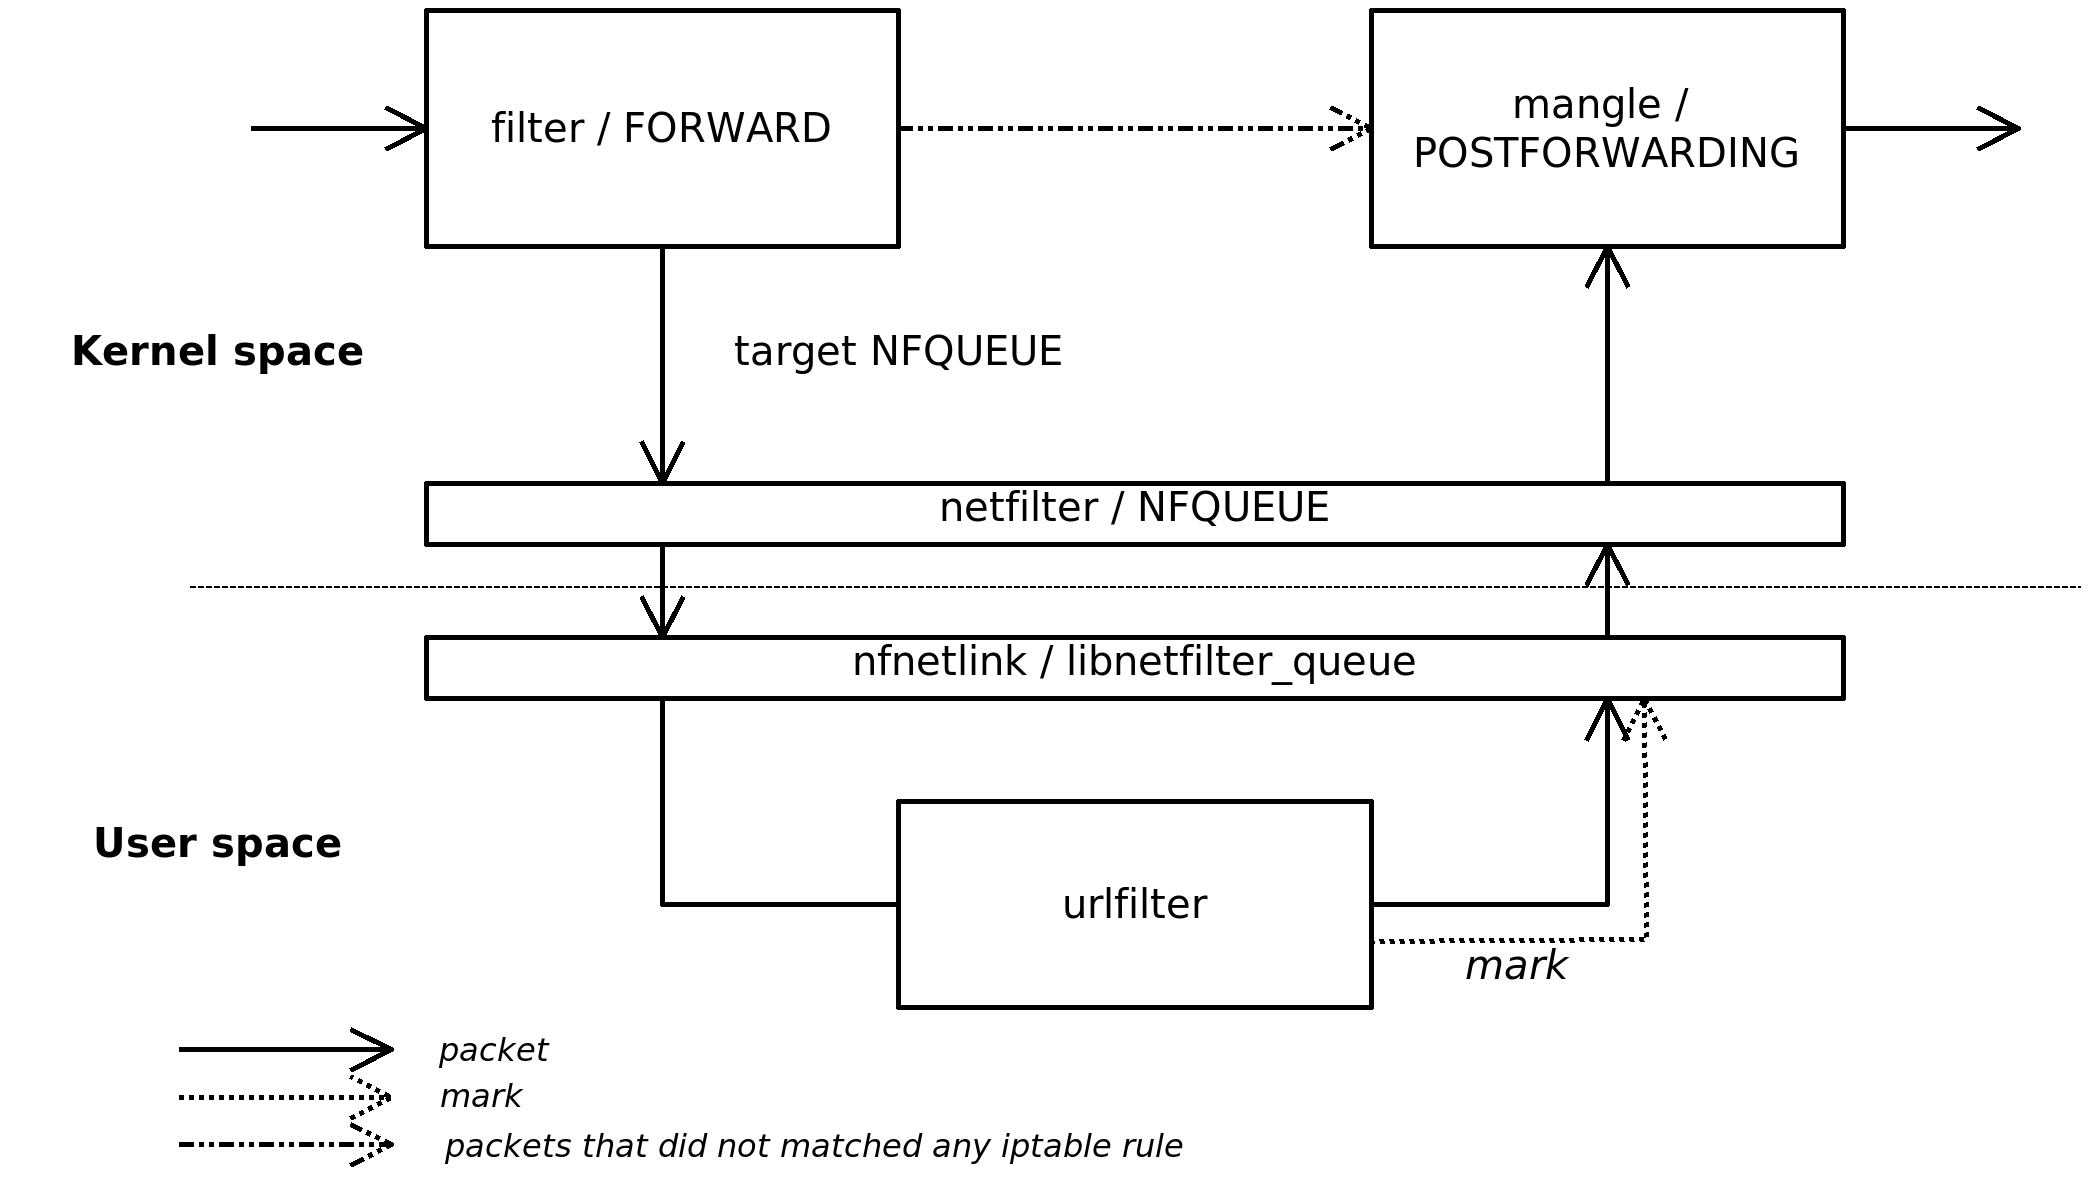
\includegraphics[scale=0.13]{pictures/schema1.png}
    \end{figure}
  \end{frame}
